\documentclass[]{article}

% ----------- BEGIN PACKAGES -----------
\usepackage[utf8]{inputenc}
\usepackage[english,serbian]{babel}
\usepackage[margin=0.7in]{geometry}
\usepackage{url}
\usepackage{float}
\usepackage[graphicx]{realboxes}
\usepackage{listings}

\usepackage{textcomp}
\usepackage{xcolor}
\usepackage{titlesec}
\usepackage{adjustbox}
\lstset {
    language=Java,
    frame=none,
    %xleftmargin=-.25in,
    %xrightmargin=.25in
    framesep=10pt,
    tabsize=4,
    showstringspaces=false,
    upquote=true,
    commentstyle=\color{black},
    keywordstyle=\color{black},
    stringstyle=\color{black},
    basicstyle=\small\ttfamily,
    emph={int,char,double,float,unsigned,void,bool},
    emphstyle={\color{black}},
    escapechar=\&,
    classoffset=1,
    morekeywords={>,<,.,;,,,-,!,=,~},
    keywordstyle=\color{black},
    classoffset=0,
    breaklines=true
}
\pagenumbering{gobble}
% ----------- END PACKAGES -----------

% ----------- BEGIN PREAMBLE -----------
\titlespacing\title{left spacing}{before spacing}{after spacing}[right]

\title{Ra\v{c}unarske mre\v{z}e 4R, Ispit - SEP1, 60p/30p}
\date{26.08.2020.}

\begin{document}

\makeatletter
\begin{center}

{\fontsize{12pt}{14pt}\selectfont\bfseries\@title\par}
\@date
\vspace{5mm}

\noindent\fbox{%
    \parbox{\textwidth}{%
      Pro\v{c}itati sve zadatke \textbf{pa\v{z}ljivo} pre rada - sve \v{s}to nije navedeno ne mora da se implementira! 

      Na \texttt{Desktop}-u se nalazi zip arhiva. Unutar arhive se nalazi direktorijum sa imenom \texttt{rm\_rok\_Ime\_Prezime\_miGGXXX}\\
      u kome se nalazi validan IntelliJ projekat. Izvu\'c{}i direktorijum iz arhive na Desktop i zameniti svojim podacima.\\
      Otvoriti IntelliJ IDEA, izabrati opciju \texttt{Open project} (ne \texttt{Import project}!) i otvoriti pomenuti direktorijum.\\ 
      Sve kodove ostaviti unutar ve\'c{} kreiranih Java fajlova. \textbf{Kodovi koji se ne prevode se ne\'c{}e pregledati.}\\
      \textbf{Nepo\v{s}tovanje formata ulaza/izlaza nosi kaznu od -10\% poena na zadatku!}
      Vreme za rad: \textbf{3h/2h}.
    }%
}
\end{center}
\makeatother
% ----------- END PREAMBLE -----------

\vspace{5pt}

% ----------- BEGIN DOCUMENT -----------
\begin{enumerate}

% ----------- BEGIN 1 -----------
\item \textbf{Non-Blocking IO (25p/18p)}
\\Za potrebe skeniranja terena odlu\v{c}eno je da se kreira \emph{hab} (server) koji \'c{}e prikupljati podatke koji se dobijaju od \emph{skenera} (klijenata). Svaki skener se odlikuje svojom pozicijom $(x,y)$ i mo\v{z}e da pokrije odgovaraju\'c{}u oblast radijusa $r$. Cilj je pokriti \v{c}itav teren skenerima. Teren se posmatra kao mre\v{z}a jedini\v{c}nih kvadrata du\v{z}ine $m$ i \v{s}irine $n$ (videti sliku ispod), dok je $(x,y)$ jedno teme mre\v{z}e. Skener pokriva kvadrat veli\v{c}ine $2r$ sa centrom u $(x,y)$. $m$, $n$, $x$, $y$ i $r$ su nenegativni celi brojevi.

\begin{figure}[h!]
  \centering
  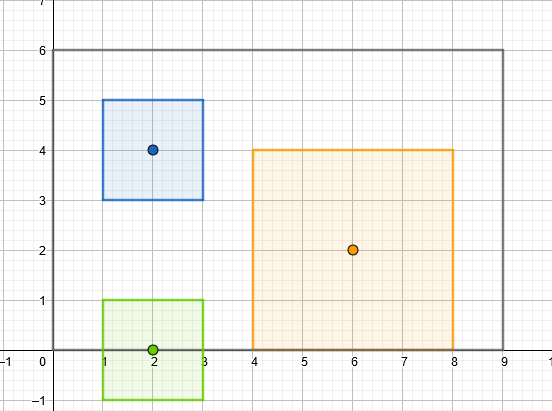
\includegraphics[scale=0.6]{images/terrain.png}
  \caption{Teren dimenzija $9 \times 6$ sa tri postavljena skenera. Pokrivenost u ovom slu\v{c}aju: $\frac{22}{9 \times 6} \approx 0.407 = 40.7\%$}
\end{figure}

\begin{itemize}
  \item Napraviti Java aplikaciju koja ima ulogu skenera. Povezati se na lokalni server na portu $7337$ koristeći \textbf{blokiraju\'c{}i Java Channels API}. Nakon formiranja konekcije, klijent serveru \v{s}alje brojeve $(x,y)$ i $r$ koje operater skenera unosi sa standardnog ulaza. Nakon slanja, klijent ispisuje odgovore od servera sve dok server ne prekine vezu. \hfill (6p/4p)
  \item Napraviti Java aplikaciju koja ima ulogu centralnog haba. Pokrenuti lokalni server na portu $7337$, koriste\'c{}i \textbf{neblokiraju\'c{}i Java Channels API}. Prilikom pokretanja, operater haba unosi veli\v{c}inu terena --- brojeve $m$ i $n$. Hab zatim opslu\v{z}uje skenere. Nakon uspostavljanja veze, hab prima podatke od skenera --- $(x,y)$ i $r$ (pozicija skenera mora biti unutar granica terena, u protivnom se raskida veza sa tim skenerom). U međuvremenu, na svakih $5$ sekundi, hab svim skenerima \v{s}alje trenutnu pokrivenost terena --- procenat jedini\v{c}nih kvadrata koji su pokriveni skenerima u odnosu na ukupan broj jedini\v{c}nih kvadrata u mre\v{z}i. \hfill (13p/9p)
  \item Server raskida vezu sa klijentima i zavr\v{s}ava sa radom onda kada pokrivenost terena postane $100\%$. \hfill (3p/2p)
  \item Obezbediti da u slučaju izuzetaka, svi resursi budu ispravno zatvoreni i da se ukupna pokrivenost terena eventualno promeni ukoliko je neki skener prekinuo vezu! \hfill (3p/3p)
\end{itemize}
% ----------- END 1 -----------

\vspace{5pt}
\begin{center}
  \textbf{------------------------------------------------------------------------------------------------------------------------------}
\end{center}
\textit{Napomena: Ohrabrujemo studente da koriste \texttt{netcat} kako bi testirali delimi\v{c}ne implementacije i otkrili gre\v{s}ke pre vremena. Takodje, ukoliko se npr. presko\v{c}i implementacija servera, mo\v{z}e se mock-ovati server putem \texttt{netcat}-a.} 
\begin{center}
  \textbf{--------------------------------------------------- Okrenite stranu! ---------------------------------------------------}
\end{center}
\newpage

% ----------- BEGIN 2 -----------
\item \textbf{UDP Sockets (20p/12p)}
\\Implementirati UDP server koji na osnovu informacija o terenu i postavljenim skenerima klijentima \v{s}alje odgovor o pokrivenosti njihove lokacije (temena mre\v{z}e terena). 
\begin{itemize}
  \item Napraviti Java aplikaciju koja ima ulogu UDP klijenta. Poslati inicijalni datagram lokalnom serveru na portu $12345$ sa lokacijom klijenta na mre\v{z}i terena (videti sliku sa prethodne strane). Ispisati \texttt{Pokriven!} ako je server odgovorio pozitivno na datagram (lokacija je pokrivena bar jednim skenerom) ili \texttt{Nije pokriven!} ukoliko je server odgovorio negativno na datagram (informacije proizvoljno kodirati u datagrame). \hfill (5p/3p)
  \item Napraviti Java aplikaciju koja ima ulogu UDP servera. Najpre iz fajla \texttt{terrain.txt} u\v{c}itati podatke o terenu i postavljenim skenerima. Primer fajla je dat ispod. \hfill (3p/2p)
  \item Nakon u\v{c}itavanja podataka o terenu, slu\v{s}ati na portu $12345$ i ispisati tekst \texttt{Pristigao klijent!} kad god server primi datagram. Odgovoriti datagramom koji sadr\v{z}i informaciju o pokrivenosti lokacije izvu\v{c}ene iz datagrama --- lokacija je pokrivena ako je u radijusu barem jednog skenera (informacije proizvoljno kodirati u datagrame). \hfill (10p/6p)
  \item Postarati se da su svi resursi ispravno zatvoreni u slu\v{c}aju izuzetka. \hfill (2p/1p)
\end{itemize}

\vspace{10pt}

\begin{figure}[h!]
  \noindent
  \begin{lstlisting}
    9 6
    3 4 1
    2 0 1
    6 2 2
  \end{lstlisting}
  \caption{Primer fajla \texttt{terrain.txt} koji odgovara slici sa prethodne strane --- u prvoj liniji se nalaze dimenzije terena, a zatim u narednim linijama se nalaze informacije o postavljenim skenerima, po jedan skener u svakoj liniji (redosled nije bitan, u ovom primeru je redosled: plavi, zeleni pa crveni).}
\end{figure}

\vspace{15pt}
Primer izvr\v{s}avanja:

\vspace{10pt}
\noindent
\begin{tabular}{ll}
\begin{lstlisting}
terrain.txt ucitan!
\end{lstlisting}& \\
\begin{lstlisting}
Server pokrenut!
\end{lstlisting}& \\
&\begin{lstlisting}
Klijent pokrenut!
\end{lstlisting}\\
&\begin{lstlisting}
> 2 1
\end{lstlisting}\\
\begin{lstlisting}
Stigao datagram!
\end{lstlisting}& \\
\begin{lstlisting}
\end{lstlisting}&\begin{lstlisting}
Pokriven!
\end{lstlisting}\\
&\begin{lstlisting}
Klijent pokrenut!
\end{lstlisting}\\
&\begin{lstlisting}
> 2 2
\end{lstlisting}\\
\begin{lstlisting}
Stigao datagram!
\end{lstlisting}& \\
\begin{lstlisting}
\end{lstlisting}&\begin{lstlisting}
Nije Pokriven!
\end{lstlisting}\\
&\begin{lstlisting}
Klijent pokrenut!
\end{lstlisting}\\
&\begin{lstlisting}
> 7 3
\end{lstlisting}\\
\begin{lstlisting}
Stigao datagram!
\end{lstlisting}& \\
\begin{lstlisting}
\end{lstlisting}&\begin{lstlisting}
Pokriven!
\end{lstlisting}\\
&\begin{lstlisting}
Klijent pokrenut!
\end{lstlisting}\\
&\begin{lstlisting}
> 100 100
\end{lstlisting}\\
\begin{lstlisting}
Stigao datagram!
\end{lstlisting}& \\
\begin{lstlisting}
\end{lstlisting}&\begin{lstlisting}
Nije Pokriven!
\end{lstlisting}\\
\end{tabular}
% ----------- END 2 -----------

\vspace{10pt}
\begin{center}
  \textbf{------------------------------------------------------------------------------------------------------------------------------}
\end{center}
\textit{Napomena: Ohrabrujemo studente da koriste \texttt{netcat} kako bi testirali delimi\v{c}ne implementacije i otkrili gre\v{s}ke pre vremena. Takodje, ukoliko se npr. presko\v{c}i implementacija servera, mo\v{z}e se mock-ovati server putem \texttt{netcat}-a.} 
\begin{center}
  \textbf{--------------------------------------------------- Okrenite stranu! ---------------------------------------------------}
\end{center}
  
% ----------- BEGIN 3 -----------
\item \textbf{Frekvencija reči (15p) (za studente koji nisu radili projekat)}
\\Napraviti Java aplikaciju koja pomoću niti broji pojavljivanja svih reči u okviru tekstualnih fajlova unutar zadatog direktorijuma.
\begin{itemize}
  \item Kao ulaz u program se daje putanja do direktorijuma (u kome može biti vi\v{s}e poddirektorijuma) u kojem se nalaze tekstualni fajlovi. Na standardni izlaz ispisati putanju do svakog regularnog fajla sa ekstenzijom \texttt{.txt} unutar tog direktorijuma kao i broj linija u svakom od pomenutih fajlova. \hfill (5p)
  \item Napraviti zajedničku stukturu podataka u kojoj će se voditi evidencija o broju pojavljivanja re\v{c}i u svim tekstualnim fajlovima unutar zadatog direktorijuma. \hfill (1p)
  \item Za svaki pomenuti tekstualni fajl, nakon ispisa broja linija u tom fajlu, pokrenuti zasebnu nit koja će, korise\'c{}i odgovaraju\'c{}e ulazne tokove podataka, da pro\v{c}ita sadr\v{z}aj tog fajla i ažurira broj pojavljivanja odgovarajućih reči u zajedničkoj strukturi podataka. \hfill (3p)
  \item Postarati se da nema konfliktnih situacija prilikom ažuriranja zajedničke strukture podataka. \hfill (3p)
  \item Na standardni izlaz ispisati sadržaj zajedničke strukture podataka sortiran opadaju\'c{}e po broju pojavljivanja u formatu \texttt{rec: brojPojavljivanja}. \hfill (2p)
  \item Postarati da su svi resursi pravilno zatvoreni u slučaju izuzetka. \hfill (1p)
\end{itemize}
% ----------- END 3 -----------

\end{enumerate}
\end{document}
% ----------- END DOCUMENT -----------

